The multi-agent path finding problem (MAPF) is more challenging than the single-agent problem due to the high dimension of its configuration space. In this chapter, we introduce the various approaches of tackling problem. 

\section{Graph Search Methods}
These approaches compute the path by applying the graph-search algorithms on the configuration space of the multi-robot system, which is the Cartesian product of the configuration spaces of each robot. Here, robot-robot collisions are expressed as configuration space obstacles. The full configuration space grows exponentially with the number of robots, thus making the standard search algorithms computationally infeasible. 

It is not necessary to plan in this space as the robots are usually well separated in the workspace, and collisions are infrequent. Some works generate feasible results by exploiting this decoupled property of the system. In this section, we discuss two such methods: M* \cite{wagner2011m} and conflict based search \cite{sharon2015conflict}. These methods have proven to produce remarkable results for cases with high congestion. 
\subsection{M* Search}
Initially, M* algorithm plans for each robot separately, without considering collisions. This is a good starting point for multi-robot planning as no path can be cheaper than this. When collisions occur, planning is performed in the joint configuration space (see Figure.~\ref{fig:mstar}) of the robots involved in the collision while uninvolved robots proceed independently. When the collision is bypassed, planning continues to proceed in low dimensional individual spaces. 

\begin{figure}
    \centering
    \begin{subfigure}[b]{0.4\textwidth}
        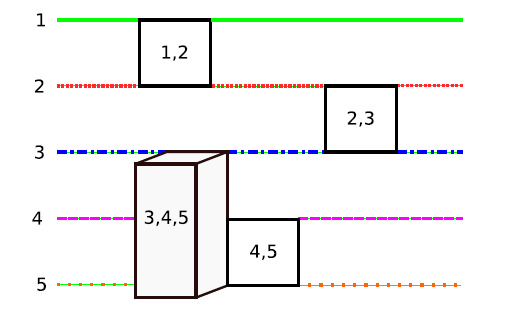
\includegraphics[width=\textwidth]{./images/m_star_a.png}
        \caption{Representation of search space in M* algorithm}
        \label{fig:mstara}
    \end{subfigure}
    ~ %add desired spacing between images, e. g. ~, \quad, \qquad, \hfill etc. 
    \begin{subfigure}[b]{0.55\textwidth}
        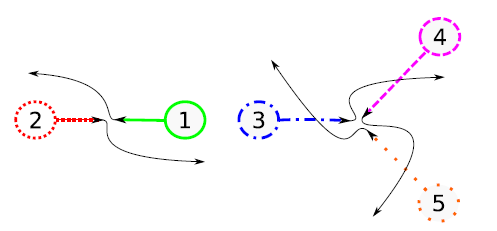
\includegraphics[width=\textwidth]{./images/m_star_b.png}
        \caption{Motion of multiple robots in the shared workspace}
        \label{fig:mstarb}
    \end{subfigure}
    \caption{Visualization of the variable dimensionality workspace in M* algorithm. When two robots collide, the local dimensionality is increased to 2 (represented by a square). Similarly, when three robots collide the dimensionality is 3 (cube). \cite{wagner2011m} }\label{fig:mstar}
\end{figure}

Like A* algorithm, M* explores a list of vertices sorted based on the sum of the cost of the cheapest path and a heuristic cost. M* considers only a limited set of neighbours determined by a \textit{collision set}, thus minimizing the dimensionality. M* can be seen as performing A* search in a  dynamically updating graph, $G^\#$. M* algorithm can handle problems involving a high number of robots, while retaining bounded optimality and \textit{completeness}. 


%M* algorithm was proven to be \textit{complete}. Moreover, it is capable of scaling to problems involving high dimension of robots, while maintaining completeness and bounded optimality. 
The uncertainties of the poses, inherent to robotics, was taken into consideration in UM* \cite{Wagner2017PathPF}. In this approach, planning is done in the belief space to account for the uncertainties. Then, a scheme similar to M* is implemented. 
\subsection{Conflict Based Search}
Conflict-Based Search (CBS) is a bounded sub-optimal two-level MAPF solver. The top level solves a binary \textit{constraint tree} (CT), whose nodes consists of a set of constraints, a single solution, and the cost of solution. The low level of CBS searches for a plan that satisfies all the constraints in a node $N$. If a node is conflict-free, it is returned as the solution. Otherwise, CBS splits node $N$ based on one of the conflicts. Let $<a_i, a_j, v, t>$ represent the conflict between agents $a_i$ and $a_j$ at vertex $v$ at time-step $t$. Now, $N$ is split into two children node, one with the constraint $<a_i, v, t>$ and the other with $<a_j,v,t>$. By doing so, the solver imposes a constraint on only one agent at a time. 

An example of this node expansion scheme is shown in Figure.~\ref{fig:cbs}. In this problem, each mouse (agent) must find a path to cheese (goal). Node $R$ is initialized with no constraints. The shortest paths generated has a collision $<1,2,D,2>$. Therefore, two nodes, $U$ and $V$, are generated with constraints $<1,D,2>$ and $<2,D,2>$ respectively. This leads to collision free solutions. As this search method is exponential in the number of conflicts encountered, as opposed to the number of agents, it leads to superior results. 

Since solving MAPF problems are optimally NP-hard, optimal solutions like M* and CBS are feasible only for low number of agents. Therefore, it is common to use bounded-suboptimal solutions for higher number of agents. Koenig et al. \cite{cohen2016bounded} uses user-provided highways to generate suboptimal paths for a large number of robots. 

The graph plans from these grid based search methods cannot be directly interpreted as trajectory results as they do not consider the kinematic and dynamics constraints of the robot. \cite{honig2016multi} deals with this problem by post-processing the output of the MAPF solvers using a simple temporal network. 

\begin{figure}
\centering
\includegraphics[width=0.6\textwidth]{./images/CBS}
\caption{Example of CBS: (I) MAPF instance, and (II) its Constraint-Tree (CT)}
\label{fig:cbs}
\end{figure}

\section{Continuous optimization schemes}
Some researchers the MAPF problem in a continuous setting by formulating it as an optimisation problem with the trajectories defined by its decision variables. These methods generate smooth solutions for small fleets of robots. 


\section{Planning with time offsets}
\section{Velocity Profile Methods}
\section{Collision Avoidance based Methods}
\subsection{Nonlinear Model Predictive Control}
\subsection{Velocity Obstacle}

\section{Spline-based refinement of Waypoints}
